\documentclass[12pt]{article}

\usepackage[margin=1in]{geometry}  
\usepackage{graphicx}              
\usepackage{amsmath}               
\usepackage{amsfonts}              
\usepackage{amsthm}                
\usepackage{amssymb}
\usepackage{mathrsfs}
\usepackage{enumerate}
\usepackage{algorithmic}
\usepackage{url}
\usepackage{tikz}
\usetikzlibrary{positioning}

%//////////////////////////////////////////////////////////////////////////////////////////////////
% theorem environments
\theoremstyle{plain}
\newtheorem{theorem}{Theorem}
\newtheorem{lemma}[theorem]{Lemma}
\newtheorem{corollary}[theorem]{Corollary}
\newtheorem{proposition}[theorem]{Proposition}

\theoremstyle{definition}
\newtheorem{definition}[theorem]{Definition}
\newtheorem{conjecture}[theorem]{Conjecture}
\newtheorem{example}[theorem]{Example}
\newtheorem*{remark}{Remark}
\newtheorem*{note}{Note}

%//////////////////////////////////////////////////////////////////////////////////////////////////

\renewcommand{\algorithmicrequire}{\textbf{Input:}}
\renewcommand{\algorithmicensure}{\textbf{Output:}}
\algsetup{linenodelimiter=.}
%% \setlength{\parindent}{0pt}


%//////////////////////////////////////////////////////////////////////////////////////////////////
% roman numerals
\newcommand{\romnum}[1]{\romannumeral #1}
\newcommand{\Romnum}[1]{\uppercase\expandafter{\romannumeral #1}}

%//////////////////////////////////////////////////////////////////////////////////////////////////

\def\gathen#1{{#1}}

% characteristic of a field
\DeclareMathOperator{\fieldchar}{char}
% endomorphism ring
\DeclareMathOperator{\ringofend}{End}
% trace of a mtrix
\DeclareMathOperator{\trace}{tr}
% Galois group
\DeclareMathOperator{\gal}{Gal}
% order of an element
\DeclareMathOperator{\order}{ord}
% least common multiple
\DeclareMathOperator{\lcm}{lcm}
% divisor on a curve
\DeclareMathOperator{\divisor}{div}
% support of a divisor
\DeclareMathOperator{\supp}{supp}
% abs
\providecommand{\abs}[1]{\left\vert#1\right\vert}

\newcommand{\leftmapsto}{\mathrel{\reflectbox{\ensuremath{\mapsto}}}}
\newcommand{\longleftmapsto}{\mathrel{\reflectbox{\ensuremath{\longmapsto}}}}

\def\N{\mathbb{N}}
\def\F{\mathbb{F}}
\def\K{\mathbb{K}}
\def\L{\mathbb{L}}
\def\M{\mathsf{M}}
\def\I{\mathsf{I}}
\def\Q{\mathsf{Q}}
\def\CC{\mathsf{C}}
\def\R{\mathsf{R}}
\def\A{\mathsf{A}}


%//////////////////////////////////////////////////////////////////////////////////////////////////
% The following allows algorithms to split over multiple pages
\makeatletter
\newcounter{algorithm}
\setcounter{algorithm}{0}
\renewcommand{\thealgorithm}{\arabic{algorithm}}
\def\algorithm{\@ifnextchar[{\@algorithma}{\@algorithmb}}
\def\@algorithma[#1]{%
  \refstepcounter{algorithm}
  \trivlist
  \leftmargin\z@
  \itemindent\z@
  \labelsep\z@
  \item[\parbox{\columnwidth}{%
    \hrule
    \hrule
    \noindent\strut\textbf{Algorithm \thealgorithm} #1
    \hrule
  }]\hfil\vskip0em%
}
\def\@algorithmb{\@algorithma[]}
\def\endalgorithm{\hfil\vskip-1em\hrule\endtrivlist}
\makeatother


\renewcommand{\qedsymbol}{$\square$}

%//////////////////////////////////////////////////////////////////////////////////////////////////

\newcommand{\keywords}[1]{\begin{description} \item[\textbf{Keywords.}] #1 \end{description}}

%//////////////////////////////////////////////////////////////////////////////////////////////////


\title{Computing Isomorphisms}
\date{}

\begin{document}

\maketitle
%\tableofcontents

\section{Introduction}

Let $F_1, F_2$ be degree $n$ extensions of the finite field $\F_p$ where $n$ is a positive integer, and $p$ is a prime number. We have an isomorphism $F_1 \simeq F_2$. Our goal is to design an efficient algorithm that provides us explicit computation of such an isomorphism.

\paragraph{Prime-degree extensions.} Although this might not be a feasible assumption, to make everything more easier and more intuitive we 
restrict ourself to extensions of prime degree. In other words, we assume for now, that we have an algorithm for computing the subfield of a given degree of a finite field. Then for an extension of degree $n$ we can write $n = r_1r_2\cdots r_k$ with $r_i$ prime, not necessarily different. Then we find subfields 
\begin{align*}
	\F_p & \subset E_1 \subset \ldots \subset E_k \subset F_1 \\
	\F_p & \subset E_1' \subset \ldots \subset E_k' \subset F_2
\end{align*}
of degrees $r_i$ for both extensions. The isomorphism tower can then be constructed inductively. 

\paragraph{Our approach.} Suppose we are given extensions $F_1, F_2$ of $\F_p$ of prime degree $r$. Our strategy of constructing an isomorphism $F_1 \simeq F_2$ is divided into the following cases.
\begin{description}
	\item[Case 1.] If $r \mid p - 1$ then there is an $r$-th root of unity in $\F_p$. We can find an element $\eta \in \F_p$ such that $X^r - \eta$ is irreducible over $\F_p$. We are then left with computing the isomorphisms $\varphi_1, \varphi_2$ in the following diagram.
	\begin{center}
		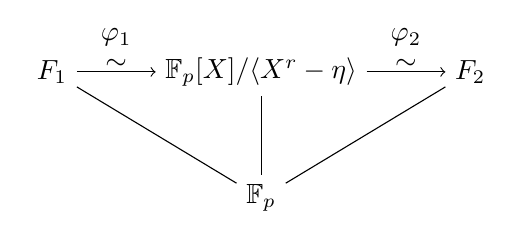
\begin{tikzpicture}
			\node (Fq) {$\F_p$};
			\node[above = of Fq] (Fqx) {$\F_p[X] / \langle X^r - \eta \rangle$};
			\node[left = of Fqx] (F1) {$F_1$};
			\node[right = of Fqx] (F2) {$F_2$};
			\draw (Fq)
				edge (F1)
				edge (F2)
				edge (Fqx);
			\draw[->] (F1) edge node[above, inner sep=0.5pt] {$ \sim $} node[above = 3mm, inner sep=0.5pt] {$ \varphi_1 $} (Fqx);
			\draw[->] (Fqx) edge node[above, inner sep=0.5pt] {$ \sim $} node[above = 3mm, inner sep=0.5pt] {$ \varphi_2 $} (F2);
		\end{tikzpicture}
	\end{center}
	To compute these isomorphisms we first compute an $r$-th root of $\eta$ in $F_1, F_2$ to get the isomorphisms
	\begin{center}
		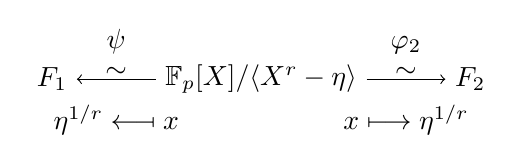
\begin{tikzpicture}
			\node (Fqx) {$\F_p[X] / \langle X^r - \eta \rangle$};
			\node[left = of Fqx] (F1) {$F_1$};
			\node[right = of Fqx] (F2) {$F_2$};
			\draw[->] (Fqx) edge node[above, inner sep=0.5pt] {$ \sim $} node[above = 3mm, inner sep=0.5pt] {$ \psi $}
				node[below = 3mm, inner sep=0.5pt] {$\eta^{1 / r} \longleftmapsto x$} (F1);
			\draw[->] (Fqx) edge node[above, inner sep=0.5pt] {$ \sim $} node[above = 3mm, inner sep=0.5pt] {$ \varphi_2 $} 
				node[below = 3mm, inner sep=0.5pt] {$x \longmapsto \eta^{1 / r}$} (F2);
		\end{tikzpicture}
	\end{center}
	Then $\varphi_1 = \psi^{-1}$ is computed using transposed modular composition.
	\item[Case 2.] If $r = p$ then Artin-Schreier theory is used.
	\item[Case 3.] If $r \nmid p - 1$ then first move to cyclotomic extensions $\F_p[\zeta], F_1[\zeta], F_2[\zeta]$. We then find an element $\eta \in \F_p[\zeta]$ that provides us isomorphisms $\varphi_1, \varphi_2$ as in the following diagram.
	\begin{center}
		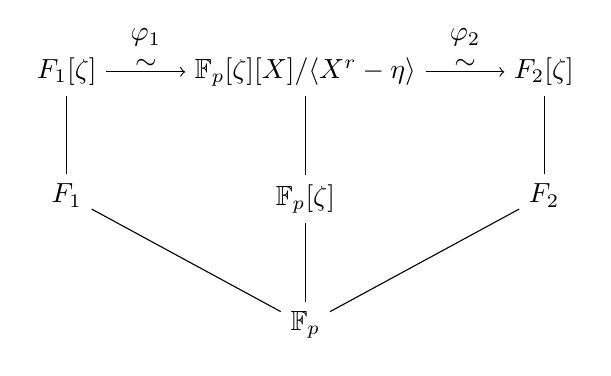
\begin{tikzpicture}
			\node (Fq) {$\F_p$};
			\node[above = of Fq] (Fqz) {$\F_p[\zeta]$};
			\node[above = of Fqz] (Fqzx) {$\F_p[\zeta][X] / \langle X^r - \eta \rangle$};
			\node[left = of Fqzx] (F1z) {$F_1[\zeta]$};
			\node[right = of Fqzx] (F2z) {$F_2[\zeta]$};
			\node[below = of F1z] (F1) {$F_1$};
			\node[below = of F2z] (F2) {$F_2$};
			\draw (Fq) edge (F1) edge (F2)	edge (Fqz)
				(Fqz) edge (Fqzx)
				(F1) edge (F1z)
				(F2) edge (F2z);
			\draw[->] (F1z) edge node[above, inner sep=0.5pt] {$ \sim $} node[above = 3mm, inner sep=0.5pt] {$ \varphi_1 $} (Fqzx);
			\draw[->] (Fqzx) edge node[above, inner sep=0.5pt] {$ \sim $} node[above = 3mm, inner sep=0.5pt] {$ \varphi_2 $} (F2z);
		\end{tikzpicture}
	\end{center}
	Then we descend $\varphi_1, \varphi_2$ down to $F_1, F_2$ respectively.
\end{description}
Throughout this note We assume the representations
\begin{equation}
\label{equation:rep}
	F_1 = \F_p[X] / \langle f(X) \rangle, \; \F_p[\zeta] = \F_p[Z] / \langle g(Z) \rangle, \;
	F_1[\zeta] = \F_p[X, Z] / \langle f(X), g(Z) \rangle
\end{equation}
where $g(Z)$ is an irreducible factor of the $r$-th cyclotomic polynomial $\Phi_r(Z)$. We also let $x, z = \zeta$ be the residue classes of $X, Z$ in these quotients.


%///////////////////////////////////////////

\section{The case $r \mid p - 1$}

We follow \cite{doliskanischost2011} to compute an $r$-th root of $\eta$ in $F_2$. Assume that $\gamma$ is an $r$-th root of $\eta$ in $F_2$. Let $\beta = T_{F_2 / \F_p}(\gamma)$, where $T_{F_2 / \F_p}:F_2 \to \F_p$ is the trace linear form. We have
\begin{align}
\label{equation:tr-simple}
\beta 
& = \sum_{i = 0}^{r - 1} \gamma^{p^i} \nonumber \\
& = \gamma(1 + \gamma^{p - 1} + \gamma^{p^2 - 1} + \cdots + \gamma^{p^{r - 1} - 1}) \nonumber \\
& = \gamma(1 + a^{(p - 1) / r} + a^{(p^2 - 1) / r} + \cdots + a^{(p^{r - 1} - 1) / r}).
\end{align}
Let $b = 1 + a^{(p - 1) / r} + a^{(p^2 - 1) / r} + \cdots + a^{(p^{(r - 1)} - 1) / r}$, so that Equation (\ref{equation:tr-simple}) gives $\beta = \gamma b$. Taking the $r$-th power in both sides gives $\beta^r = ab^r$ over $\F_p$. We then can compute $\beta$ by an $r$-th root extraction in $\F_p$. If we assume that $b \ne 0$ (or equivalently that $\beta \ne 0$), we deduce $\gamma = \beta b^{-1}$; in case $\beta$ is zero, we replace $a$ by $a'=ac^r$, for a nonzero random $c \in F_2$. By Proposition 3 in \cite{doliskanischost2011} all these take $O(\M(r)\log(p) + \CC(r)\log(r))$ operations in $\F_p$.




%///////////////////////////////////////////

\section{The case $r \nmid p - 1$}

In this section we assume that $r \nmid p - 1, r \ne p$. Let $s$ be the order of $p$ in $\mathbb{Z} / r\mathbb{Z}$, and write $p^s - 1 = ur^t$ where $\gcd(r, u) = 1$. To mimic Case 1 above, we can find a non-$r$-adic residue $\eta$ in $\F_p[\zeta]$, construct the extension $\F_p[\zeta][X] / \langle X^r - \eta \rangle$, and finally compute an $r$-th root of $\eta$ in $F_1, F_2$. But, as a more efficient way, we show how to do all these at once while skipping some detail computations. We first need the following result.
\begin{proposition}
\label{proposition:semi-trace}
	For an element $a \in F_1[\zeta]$ define 
	\begin{equation}
	\label{equation:semi-trace} 
		\theta_a = a + \zeta^{r - 1}a^{p^s} + \cdots + \zeta^2a^{p^{(r - 2)s}} + \zeta a^{p^{(r - 1)s}}
	\end{equation}
	Then
	\begin{enumerate}
		\item[\normalfont (i)] There is an $a \in F_1[\zeta]$ such that $\theta_a \ne 0$.
		\item[\normalfont (ii)] $\theta_a, \theta_a^r$ are non-$r$-adic residues in $F_1[\zeta], \F_p[\zeta]$ respectively.
	\end{enumerate}
\end{proposition}
\begin{proof}
	Let $v = u^{-1} \bmod r$, and let $\gamma \in F_1[\zeta]$ be an $r^t$-th root of $\zeta^{v(r - 1)}$. There exists an element $a \in F_1[\zeta]$ such that $\beta = T_{F_1[\zeta] / \F_p[\zeta]}(\gamma a) \ne 0$, and we have
	\begin{equation}
	\label{equation:trace}
		\begin{aligned}
			\beta 
			& = \gamma a + (\gamma a)^{p^s} + \cdots + (\gamma a)^{p^{(r - 1)s}} \\
			& = \gamma (a + \gamma^{p^s - 1}a^{p^s} + \cdots + \gamma^{p^{(r - 1)s} - 1}a^{p^{(r - 1)s}}) \\
			& = \gamma (a + \gamma^{ur^t}a^{p^s} + \cdots + \gamma^{ur^t(p^{(r - 2)s} + \cdots + p^s + 1)}a^{p^{(r - 1)s}}) \\
			& = \gamma (a + \zeta^{r - 1}a + \cdots + \zeta a^{p^{(r - 1)s}}) \\
			& = \gamma \theta_a.
		\end{aligned}
	\end{equation}
	This proves (i). To prove (ii), first observe that $\theta_a^{p^s} = \zeta\theta_a$ so that $\sigma(\theta_a) = \zeta\theta_a$ for a generator $\sigma: x \to x^{p^s}$ of $\gal(F_1[\zeta] / \F_p[\zeta])$. Therefore, we have $\sigma(\theta_a^r) = \theta_a^r$, which means that $\theta_a^r \in \F_p[\zeta]$, and $\theta_a^{ur^t} = \theta_a^{p^s - 1} = \zeta$ which proves that $\theta_a, \theta_a^r$ are non-$r$-adic residues.
\end{proof}

Let $\eta_a = \theta_a^r, \eta_b = \theta_b^r$ for nonzero $\theta_a, \theta_b$ as in Proposition \ref{proposition:semi-trace}. Then we can construct isomorphisms $\varphi_1, \varphi_2$ as in the following diagram.
\begin{equation}
\label{equation:iso-chain}
	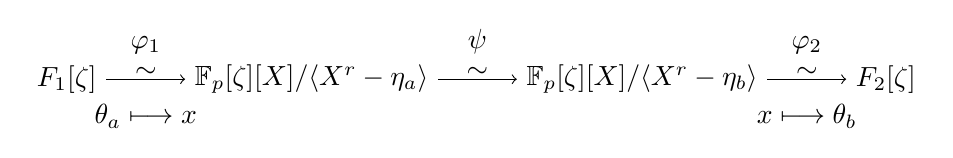
\begin{tikzpicture}
		\node (Fpzxa) {$\F_p[\zeta][X] / \langle X^r - \eta_a \rangle$};
		\node[right = of Fpzxa] (Fpzxb) {$\F_p[\zeta][X] / \langle X^r - \eta_b \rangle$};
		\node[left = of Fpzxa] (F1z) {$F_1[\zeta]$};
		\node[right = of Fpzxb] (F2z) {$F_2[\zeta]$};
		\draw[->] (F1z) edge node[above, inner sep=0.5pt] {$ \sim $} node[above = 3mm, inner sep=0.5pt] {$ \varphi_1 $}
			node[below = 3mm, inner sep=0.5pt] {$\theta_a \longmapsto x$} (Fpzxa);
		\draw[->] (Fpzxa) edge node[above, inner sep=0.5pt] {$ \sim $} node[above = 3mm, inner sep=0.5pt] {$ \psi $} (Fpzxb);
		\draw[->] (Fpzxb) edge node[above, inner sep=0.5pt] {$ \sim $} node[above = 3mm, inner sep=0.5pt] {$ \varphi_2 $}
			node[below = 3mm, inner sep=0.5pt] {$x \longmapsto \theta_b$} (F2z);
	\end{tikzpicture}
\end{equation}
To complete this isomorphism chain, we need to compute $\psi$. For that we simply compute an $r$-th root of $\eta_a$ in $E = \F_p[\zeta][X] / \langle X^r - \eta_b \rangle$, and construct the isomorphism in the obvious way. Note that from (\ref{equation:trace}) we have $\beta_a = \gamma_a\theta_a$,  $\beta_b = \gamma_b\theta_b$, and we can choose $\gamma_a, \gamma_b$ such that $\gamma_a^r = \gamma_b^r$. Therefore,
\[ \eta_a\eta_b^{-1} = \beta_a^r\beta_b^{-r} = (\beta_a\beta_b^{-1})^r = c^r. \]
So we can construct the isomorphism
\begin{equation*}
	\begin{array}{rrll}
		\psi: & \F_p[\zeta][X] / \langle X^r - \eta_a \rangle & \longrightarrow & \F_p[\zeta][X] / \langle X^r - \eta_b \rangle \\
		& x & \longmapsto & cx
	\end{array}
\end{equation*}
by computing an $r$-th root in $\F_p[\zeta]$.




%---------------------------------------------------

\subsection{Computing $\theta_a$}

Let $a \in F_1[\zeta]$. To compute $\theta_a$, we use a binary powering scheme similar to the one in \cite{doliskanischost2011}. Assuming the representations (\ref{equation:rep}) we let 
\[
\xi_i = x^{p^{is}}, \quad
\delta_i = a + z^{r - 1}a^{p^s} + \cdots + z^2a^{p^{(i - 1)s}} + z^{r - i + 1} a^{p^{(i - 1)s}}.
\]
Then we have the following relations:
\[\xi_1 = x^{p^s}, \quad \delta_1 = a, \]
\[
\xi_i =
\begin{cases}
\xi_{i / 2}^{p^{is / 2}} & \text{if $i$ is even}  \\
\xi_{i - 1}^{p^s} & \text{if $i$ is odd,}
\end{cases} \quad
\delta_i=
\begin{cases}
	z^{r - i / 2}\delta_{i / 2}^{p^{is / 2}} + \delta_{i / 2} & \text{if $i$ is even} \\
	z^{r - 1}\delta_{i - 1}^{p^s} + \delta_1 & \text{if $i$ is odd}
\end{cases}
\]
Assuming $\xi_i = x^{p^{is}}$ is already known, $\delta_i$ can be computed using the following algorithm.

\begin{algorithm}
[XiDelta$(i, \xi_1,\zeta_1)$]
\label{algorithm:xidelta}
	\begin{algorithmic}[1]
		\REQUIRE a positive integer $i$, $\xi_1 = x^{p^s}$, $\zeta_1 = a$
		\ENSURE $\xi_i$, $\delta_i$
		\IF {$i=1$} 
			\RETURN $\xi_1$, $\zeta_1$
		\ENDIF
		\STATE $j \leftarrow \lfloor i/2\rfloor$
		\STATE $\xi_{j}, \delta_j \leftarrow {\rm XiDelta}(j,\xi_1,\zeta_1)$ 
		\STATE\label{step:xi} $\xi_{2j} \leftarrow \xi_j(\xi_j)$
		\STATE\label{step:delta} $\delta_{2j} \leftarrow z^{r - j}\delta_j(\xi_j) + \delta_j$
		\IF {$i$ is even} 
			\RETURN $\xi_{2j}$, $\delta_{2j}$
		\ENDIF
		\STATE $\xi_i \leftarrow \xi_{2j}(\xi_1)$
		\STATE $\delta_i \leftarrow z^{r - 1}\delta_j(\xi_1) + \delta_1$
		\RETURN $\xi_i$, $\delta_i$
	\end{algorithmic}
\end{algorithm}

The following proposition is deduced from Algorithm \ref{algorithm:xidelta}.
\begin{proposition}
\label{proposition:XiDelta}
	For an element $a \in F_1[\zeta]$, $\theta_a$ can be computed using $O(\CC(r)\log(r) + rM(s)\log(r) + \M(r)\log(p))$ operations in $\F_p$.
\end{proposition}
\begin{proof}
	To compute the initial value $\xi_1 = x^{p^s}$ we first compute $x^p$, and then do $\log(s)$ modular compositions at a total cost of $O(\M(r)\log(p) + C(r)\log(s))$ operations in $\F_p$. Then $\theta_a = \delta_r$ is computed using Algorithm \ref{algorithm:xidelta}: the complexity of the algorithm is dominated by steps \ref{step:xi}, \ref{step:delta}. The former takes $C(r)$ operations in $\F_p$, and the later is done by evaluating $\delta_i$ at $\xi_i$ using the Horner's method at a cost of $O(r\M(s))$ operations in $\F_p$. Accounting for a recursion depth of $\log(r)$, the running time of the algorithm is then $O(\CC(r)\log(r) + rM(s)\log(r))$ operations in $\F_p$. All in all, we get the claimed complexity.
\end{proof}




%---------------------------------------------------

\subsection{Computing $r$-th roots in $\F_p[\zeta]$}
\label{subsection:rth-root-fpz}

Let $a \in \F_p[\zeta]$ be an $r$-th power. To compute an $r$-th root of $a$ we factor the polynomial $X^r - a$ using the Equal Degree Factorization algorithm given in \cite{kaltofen1997fast}.

\begin{algorithm}
[Root Finding]
\label{algorithm:edf}
	\begin{algorithmic}[1]
		\REQUIRE a square-free polynomial $f \in \F_p[\zeta][x]$ of degree $n$ with linear factors
		\ENSURE a single factor of $f$
		\IF {$\deg f = 1$}
			\RETURN $f$
		\ENDIF
		\STATE Pick a random element $\alpha \in \mathbb{A}_f = \F_p[\zeta][x]/\langle f \rangle$
		\STATE\label{step:edf-trace} Compute the following trace in $\mathbb{A}_f$
			\[ \beta = \alpha + \alpha^p + \alpha^{p^2} + \cdots + \alpha^{p^{s - 1}} \]
		\STATE $\gamma \leftarrow \beta^{(p - 1) / 2}$
		\STATE $g \leftarrow \gamma \bmod f$, $g_1 \leftarrow \gcd(g, f)$, $g_2 \leftarrow \gcd(1 + g, f)$
		\STATE Recursively factor one of $g_1, g_2$ that is non-constant
	\end{algorithmic}
\end{algorithm}

The dominant cost of the algorithm comes from Step \ref{step:edf-trace}, which is done as follows. Let
\[ \beta_i = \alpha^p + \alpha^{p^2} + \cdots + \alpha^{p^i}, \quad \xi_i = x^{p^i}, \quad \zeta_i = z^{p^i}. \]
Then we have $\beta_1 = \alpha^p$, $\xi_1 = x^p$, $\zeta_1 = z^p$, and
\[
\beta_j = 
\begin{cases}
	\beta_{j / 2} + \beta_{j / 2}^{p^{j / 2}} & j \text{ even} \\
	\beta_1 + \beta_{j - 1}^p & j \text{ odd}
\end{cases}, \quad
\xi_j = 
\begin{cases}
	\xi_{j / 2}^{p^{j / 2}} & j \text{ even} \\
	\xi_{j - 1}^p & j \text{ odd}
\end{cases}, \quad
\zeta_j = 
\begin{cases}
	\zeta_{j / 2}^{p^{j / 2}} & j \text{ even} \\
	\zeta_{j - 1}^p & j \text{ odd}
\end{cases}
\]
For a positive integer $j$ we have
\begin{equation}
\label{equation:betaj}
	\beta_j^{p^j} = \left( \sum_{l = 0}^{n - 1}c_l(z)x^l \right)^{p^j} = \sum_{l = 0}^{n - 1}c_l(z^{p^j})(x^{p^j})^l = \sum_{l = 0}^{n - 1}c_l(\zeta_j)\xi_j^l.
\end{equation}
Therefore we have a recursive algorithm for computing $\beta = \beta_{s - 1}$. Let us analyze the complexity of the algorithm. First note that we always have $z^r = 1, x^r = a$. This makes it possible to keep the identities simple and do the reductions at the end of each step. For example $x^p = a^{\lfloor p / r\rfloor}x^{p \bmod r}$ which can be computed using $O(\M(s)\log(p))$ operations in $\F_p$. At step $j$ of the recursion we have the following costs in $\F_p$:
\begin{itemize}
	\item $O(\M(r) + \M(s)\log(r))$ for computing $x^{p^j}$, and computing $z^{p^j}$ is free.
	\item $O(n\M(r))$ for reducing coefficients $c_l(z)$ of (\ref{equation:betaj}) modulo $g(z)$.
	\item $O(n\M(s))$ for evaluating $\beta_j$ at $x^{p^j}$ using Horner's method.
	\item $O(\M(r)\M(s))$ for reducing (\ref{equation:betaj}) modulo $f$.
\end{itemize}
The depth of the recursion is $\log(s)$, hence $\beta$ can be computed in 
\[O(\M(s)\log(p) + n\M(r)\log(s) + \M(r)\M(s)\log(s)) \]
operations in $\F_p$. Finally since the depth of the recursion in Algorithm \ref{algorithm:edf} is $\log(r)$, the total cost of root finding in $\F_p[\zeta]$ is 
\[ O(\M(s)\log(p)\log(r) + r\M(r)\log(s) + \M(r)\M(s)\log(s)\log(r)). \]


%---------------------------------------------------

\subsection{Computing the isomorphism $F_1 \rightarrow F_2$}

In this section, we analyze the computational cost of building an isomorphism $\varphi: F_1 \rightarrow F_2$. We first construct the isomorphism $\varphi_2 \circ \psi \circ \varphi_1 : F_1[\zeta] \rightarrow F_2[\zeta]$ as in (\ref{equation:iso-chain}), and then descend back to the desired fields. The following algorithm builds the above chain of isomorphism based on the observations at the start of the section. 

\begin{algorithm}
[Isomorphism ${F_1[\zeta] \rightarrow F_2[\zeta]}$]
\label{algorithm:ext-iso}
	\begin{algorithmic}[1]
		\REQUIRE degree $r$ extensions $F_1, F_2$ of $\F_p$
		\ENSURE an isomorphism $F_1[\zeta] \rightarrow F_2[\zeta]$
		\STATE\label{step:factor-cyclo} factor the cyclotomic polynomial $\Phi_r(Z)$ over $\F_p$ to build extensions $\F_p[\zeta], F_1[\zeta], F_2[\zeta]$
		\REPEAT
			\STATE choose a random $a \in F_1[\zeta]$
			\STATE compute $\theta_a$ using Algorithm \ref{algorithm:xidelta}
		\UNTIL {$\theta_a \ne 0$}
		\REPEAT
			\STATE choose a random $b \in F_2[\zeta]$
			\STATE compute $\theta_b$ using Algorithm \ref{algorithm:xidelta}
		\UNTIL {$\theta_b \ne 0$}
		\STATE\label{step:gamma-pow} $\eta_a \leftarrow \theta_a^r$ , $\eta_b \leftarrow \theta_b^r$
		\STATE\label{step:psi} construct the isomorphism $\psi$ as in (\ref{equation:iso-chain})
		\STATE construct $F_1[\zeta] \rightarrow F_2[\zeta]$ as in (\ref{equation:iso-chain})
	\end{algorithmic}
\end{algorithm}

\begin{proposition}
	Algorithm \ref{algorithm:ext-iso} computes the isomorphism $F_1[\zeta] \rightarrow F_2[\zeta]$ in
	\[ O(\M(r)\log(p) + \M(s)\log(p)\log(r) + r\M(r)\log(s) + \M(s)\M(r)\log(s)\log(r)) \]
	operations in $\F_p$.
\end{proposition}
\begin{proof}
	By \cite[Theorem 9]{shoup1994fast} Step \ref{step:factor-cyclo} takes $O(r\log^2(r) + r\log(r)\log(p))$ operations in $\F_p$. Finding a nonzero $\theta_a$ for a random $a \in F_1[\zeta]$ requires $O(1)$ trials, so the two repeat...until loops take $O(\CC(r)\log(r) + rM(s)\log(r) + \M(r)\log(p))$ operations in $\F_p$ by Proposition \ref{proposition:XiDelta}. Step \ref{step:gamma-pow} is done using $O(\M(s)\M(r)\log(r))$ operations in $\F_p$. Step \ref{step:psi} takes $O(\M(s)\log(p)\log(r) + r\M(r)\log(s) + \M(r)\M(s)\log(s)\log(r))$ as explained in Subsection \ref{subsection:rth-root-fpz}. Adding all these up proves the proposition.
\end{proof}

So, now we have an isomorphism $\phi: F_1[\zeta] \rightarrow F_2[\zeta]$ that sends $\theta_a$ to some $h(z, x) \in F_2[\zeta]$. To construct the isomorphism $\varphi: F_1 \rightarrow F_2$ we the technique in \cite{Allombert2002}. Let 
\[ \theta_a = \sum_{i = 0}^{s - 1}f_i(x)z^i, \quad\text{and}\quad z^s = (v(z)  \bmod g(z)) = \sum_{i = 0}^{s - 1}v_iz^i. \] 
Then since $\theta_a^{p^s} = z\theta_a$ we have
\[ \sum_{i = 0}^{s - 1}f_i(x)^{p^s}z^i = f_{s - 1}(x)v(z) + f_0(x)z + \cdots + f_{s - 2}(x)z^{s - 1}.\]
After rearranging the terms in the right hand side, this gives us the identities
\[
\begin{array}{ccc}
f_0(x)^{p^s} & = & v_0f_{s - 1}(x) \\
f_1(x)^{p^s} & = & f_0(x) + v_1f_{s - 1}(x) \\
\vdots & \vdots & \vdots \\
f_{s - 1}(x)^{p^s} & = & f_{s - 2}(x) + v_{s - 1}f_{s - 1}(x)
\end{array} 
\]
form which we see that $f_i(x) \in \F_p(f_0(x)) \subseteq F_1$ for all $i$. We prove $\F_p(f_0) = F_1$. Let $\sigma \in \gal(F_1(z) / \F_p)$ be a generator, and let $j \le r$ be the smallest integer such that $\sigma^jf_0 = f_0$. Then $\sigma^{js}\theta_a = \theta_a$, but $\theta_a$ is not contained in any proper subfield; so $j = r$. Let $h_0$ be the constant term of $h(z, x)$. Then we similarly have $F_2 = \F_p(h_0)$. This gives us an isomorphism
\[
\begin{array}{rlll}
	\phi: & F_1 & \longrightarrow & F_2 \\
	& f_0 & \longmapsto & h_0
\end{array}
\]
from which we can get an isomorphism
\[
\begin{array}{rlll}
	\phi: & F_1 & \longrightarrow & F_2 \\
	& x & \longmapsto & a(x)
\end{array}
\]
using transposed modular composition. 


\addcontentsline{toc}{section}{References}
\bibliographystyle{plain}
\bibliography{references}

\end{document}
